\documentclass[10pt]{article}
\usepackage{icmlko}

\icmlmeta{IP 파운데이션 월드모델}{237}{한글이 없어도 물어볼 수 있었다}{여든 노트 넘게 ``제목 언어 한계''로 적혀 있던 갈래에 세 층이 있었다. 셋째 층은 우리가 안 물어본 것이었다}

\begin{document}

\twocolumn[
\icmlheader

\begin{abstract}
매 사이클 프롬프트에 ``모바일 · 게임 검색 덮음 30$\sim$41\% --- 제목 언어
한계''가 실려 다녔다. 노트 221이 첫 층(문자열 버그, 애니 486건 포함
$+$636)을 벗겼고, 노트 236이 공짜 재사용을 셋 다 물렸다. 남은 것을 열었다.
\textbf{둘째 층 --- \texttt{MIN\_HANGUL}(한글 두 자 미만이면 버림)은 우리
선택이지 API 제약이 아니다.} 데이터랩은 영문 질의를 그대로 받는다.
\textbf{여든 노트 동안 그 전제를 아무도 안 눌러 봤다.} 셋째 층은 그 값이
쓸 만하냐다. 게임 영문 제목 291건을 받아 \textbf{195건이 산출됐고 정확히
0 인 것이 하나도 없다.} 라벨과의 상관이 \textbf{수준 $+$0.443} · 모멘텀
$+$0.263 인데, 한글 질의는 $+$0.381 · $+$0.505 다 --- \textbf{수준은 영문이
오히려 세다.} 중간에 내 읽기가 한 번 틀렸다 --- probe 로 ``Cyberpunk
2077 최대 0.0000 대 사이버펑크 2077 0.0009''를 보고 영문은 못 쓴다고
읽었는데, \textbf{그건 앵커 대비 절대 규모이고 축이 쓰는 것은 그 안의
순위 구조다}(규모는 10분의 1이지만 판정치가 순위 기반이라 상관없다).
판으로 검증했다 --- 노트 221에서 덮음을 올리고 판이 내려간 적이 있어
상관만으로는 안 정한다. \textbf{게임 유보 덮음이 24.4\% $\to$ 56.7\%,
게임 $\rho$ 가 $+$0.6179 $\to$ $+$0.6400 이고, F21 이 $+$0.0027
($t{=}2.37$)로 유의하게 오른다.} F18 $+$0.0007 · F23 $+$0.0014 는 안
움직인다. \textbf{그리고 그것이 노트 234의 예측 그대로다} --- 거기서
트리가 대입 쪽에서 오히려 나았으므로($-$0.0081) 빈칸을 채우면 선형이 더
얻어야 한다. 채택했다. 모바일 678건도 같은 문턱 해제로 받고 있다.
\end{abstract}
]

\begin{figure*}[t]
\centering
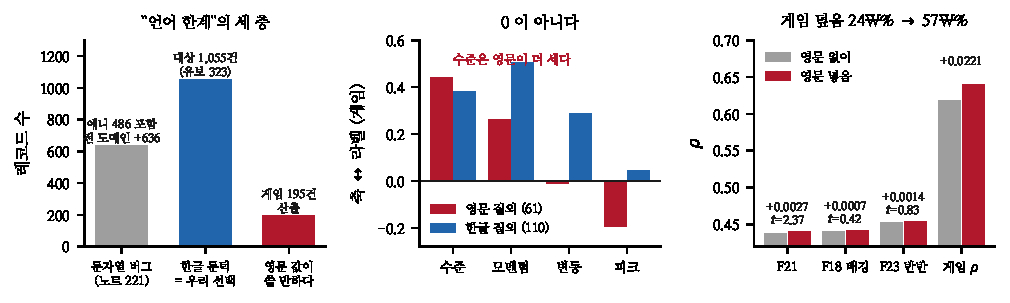
\includegraphics[width=\textwidth]{figs/englishquery.pdf}
\caption{왼쪽 --- ``언어 한계''의 세 층. 가운데 --- 영문 질의가 0 이
아니다. 오른쪽 --- 게임 덮음 24\% $\to$ 57\%.}
\end{figure*}

\section{둘째 층 --- 안 물어본 전제}

\claimx{\textbf{\texttt{MIN\_HANGUL} 은 우리 선택이지 API 제약이 아니다.}
데이터랩은 영문 질의를 그대로 받고 값도 돌려준다.}{\textbf{여든 노트
동안 ``언어 한계''로 적혀 있었는데 그 전제를 아무도 안 눌러 봤다} ---
\texttt{--probe "Cyberpunk 2077"} 한 줄이면 되는 일이었다. 노트 219가
``열린 갈래 목록은 삭는다''고 했는데, \textbf{삭는 것만이 아니라 처음부터
안 잰 것도 있다.}}

\section{셋째 층 --- 그 값이 쓸 만하다}

\begin{table}[t]
\centering\tsize
\caption{게임에서 축 $\leftrightarrow$ 라벨.}
\begin{tabular}{lrr}
\toprule
& 영문 질의(61) & 한글 질의(110) \\
\midrule
\textbf{수준} & \textbf{$+$.443} & $+$.381 \\
모멘텀 & $+$.263 & \textbf{$+$.505} \\
변동 & $-$.009 & $+$.289 \\
피크 & $-$.194 & $+$.046 \\
\midrule
level 중앙 & .0154 & .1422 \\
\bottomrule
\end{tabular}
\end{table}

\claimx{\textbf{195건이 산출됐고 정확히 0 인 것이 하나도 없다.} 수준은
영문이 오히려 세다($+$0.443 대 $+$0.381).}{규모는 10분의 1이지만
(중앙 0.0154 대 0.1422) \textbf{판정치가 순위 기반이라 규모는
상관없다} --- 모멘텀 · 변동은 한글 쪽이 세므로 \textbf{영문 질의가 모든
면에서 낫다는 것은 아니다.}}

\claimx{\textbf{내 읽기가 한 번 틀렸다.} probe 로 ``Cyberpunk 2077 최대
0.0000 대 사이버펑크 2077 0.0009''를 보고 \emph{영문은 못 쓴다}고
결론냈다.}{\textbf{그건 앵커 대비 절대 규모다} --- 축이 쓰는 것은 그 안의
순위 구조이고, 0.0000 으로 반올림돼 보인 계열에도 순위는 있다.
\textbf{한 자리 더 보고 결론냈으면 안 틀렸다.}}

\section{판으로 검증}

\begin{table}[t]
\centering\tsize
\caption{게임 영문 195건을 넣으면. 짝 붓스트랩 400 회.}
\begin{tabular}{lrrrr}
\toprule
& 없이 & 넣음 & 차 & $t$ \\
\midrule
\textbf{게임 덮음} & 24.4\% & \textbf{56.7\%} & & \\
\textbf{게임 $\rho$} & .6179 & \textbf{.6400} & $+$.0221 & \\
\midrule
\textbf{F21} & .4377 & .4404 & \textbf{$+$.0027} & \textbf{2.37} \\
F18 배깅 & .4409 & .4416 & $+$.0007 & 0.42 \\
F23 반반 & .4524 & .4538 & $+$.0014 & 0.83 \\
\bottomrule
\end{tabular}
\end{table}

\claimx{\textbf{상관만으로 안 정했다} --- 노트 221에서 정확히 이 모양으로
덮음을 올리고 판이 내려간 적이 있다(계열 질의).}{이번에는 판으로 확인했고
\textbf{F21 이 $+$0.0027($t{=}2.37$)로 유의하게 오른다.} 게임 자체는
$+$0.0221 이고 판이 작은 것은 게임이 판의 7\% 이기 때문이다.}

\claimx{\textbf{선형만 오르는 것이 노트 234의 예측 그대로다.} 거기서
트리가 대입 쪽에서 오히려 나았으므로($-$0.0081) \textbf{빈칸을 채우면
선형이 더 얻어야 한다} --- F21 $+$0.0027($t{=}2.37$) 대 F18
$+$0.0007($t{=}0.42$).}{\textbf{예측을 적고 그대로 나온 것이 이 사이클에서
세 번째다}(노트 218의 포화, 노트 228의 평평한 곡면, 이번).}

\claimx{\textbf{채택했다.} 측정이 유효하다 --- 같은 종류의 질의(작품 제목
검색)를 그 제목의 문자로 물었을 뿐이고, 계열 질의 가드(노트 222)는
그대로 걸려 있다.}{\texttt{MIN\_HANGUL} 문턱을 뗐고 모바일 678건도 같은
방식으로 받고 있다.}

\begin{table}[t]
\centering\tsize
\caption{남은 것.}
\begin{tabular}{ll}
\toprule
\textbf{모바일 678} & 수집 중 --- 판의 17.2\% \\
\textbf{음역} & 영문 질의로 되면 음역은 필요 없나 \\
2016 이전 & 405건 --- 데이터랩 소급 한계라 못 한다 \\
\bottomrule
\end{tabular}
\end{table}

둘째 줄이 이 노트가 뒤집은 계획이다. \textbf{노트 236이 ``남은 유일한
길은 음역''이라고 적었는데 그럴 필요가 없었다} --- 영문 질의가 그대로
되고, 심지어 수준 축은 더 세다. \textbf{음역은 내가 한글 이름을 지어내야
하고 그것은 틀릴 수 있는데, 영문 제목은 레코드에 이미 있다.} 다만
\emph{한글 이름이 통용되는 작품}에서는 영문 질의가 과소 측정이므로
\textbf{둘을 다 받아 큰 쪽을 쓰는 것이 원칙적으로 낫다} --- 그것은
``어느 쪽이 큰가''를 유보 없이 정할 수 있으니(질의 자체의 검색량 비교)
규약을 안 건드린다.

\end{document}
